\section{Proposed system}
The proposed system is client-server calendar application capable of syncing with other calendar servers. It’s able to have entries for one or multiple persons. Persons are part of workgroups, making it easier to manage large entries, since it’s possible to invite a workgroup instead of all individual persons.
\subsection{Functional requirements}
The system supports two kind of users:
\begin{description}
\item [The User:] Able to manage entries in the calendar, which includes creating, updating and deleting entries. It should also be possible to add other users to the entry, during creation and after.
\item [The Administrator:] Able to manage accounts, which include creating, updating and deleting entries. An administrator should also be able to create, update and delete workgroups.
\end{description}
\subsection{Nonfunctional requirements}

\begin{center}
    \begin{tabular}{ | l | p{10cm} |}
    \hline
    Category & Nonfunctional requirements \\ \hline
    Usability & The UI of the client must resemble a paper calendar to ease the learning process.\\ \hline
    Reliability & Loss of connection to the server must only cut off functions requiring connection, but not access to information already loaded.\\ \hline
    Performance & \tabitem The server must support multiple clients at once, a minimum of 1000 should be able to use the system at the same time. \\
    \mbox{} & \tabitem The communication between client and server, should at most take 2 seconds when managing a entry. The communication should take at most 10 seconds when syncing with google. \\ \hline
	Supportability & ... \\ \hline
	Implementation & The system should be implemented in C\# and work on all newer versions of Windows. \\ \hline
	Operation & ... \\ \hline
	Legal & ... \\ \hline
    \end{tabular}
\end{center}
\subsection{System models}

\subsubsection{Scenarios}
\textbf{Scenario name:} accountForNewUser
\\
\textbf{Participating actors:} Jon:User, Ben:Administrator
\\
\textbf{Flow of events:}
\begin{itemize}
\item Jon joins the firm, and thus requires access the the calendar system.
\item He contacts Ben, the administrator, by mail or in person to ask for access.
\item Ben registers a new account in the calendar system for Jon.
\item Ben puts Jons new account in all relevant workgroups, such as the workgroup for Jons department, the whole workplace etc.
\item Ben contacts Jon with the login and now Jon has access to the calendar system

\end{itemize}
\textbf{Scenario name:} createEntryForMeeting
\\
\textbf{Participating actors:} Jon:User, Mette:User
\\
\textbf{Flow of events:}
\begin{itemize}
\item Jon wants to hold a meeting and as such he starts to create an entry in his calendar filling in the information regarding time and date, and subject.
\item Since the meeting is for a group of people, Jon wants everyone going to the meeting to see it in their calendar. Thus he invites Mette, and the the people from his department, the workgroup HR.
\item Jon then creates the entry, causing the system to show the entry in all invited persons calendar along with a notification.
\item Mette unfortunately has another appointment at the time and dismiss the entry, removing it from her calendar.
\item The entry is then updated to show who is able to come.

\end{itemize}
\pagebreak
\subsubsection{Use case model}
Below is the use case model
\begin{figure}[h]
\centering
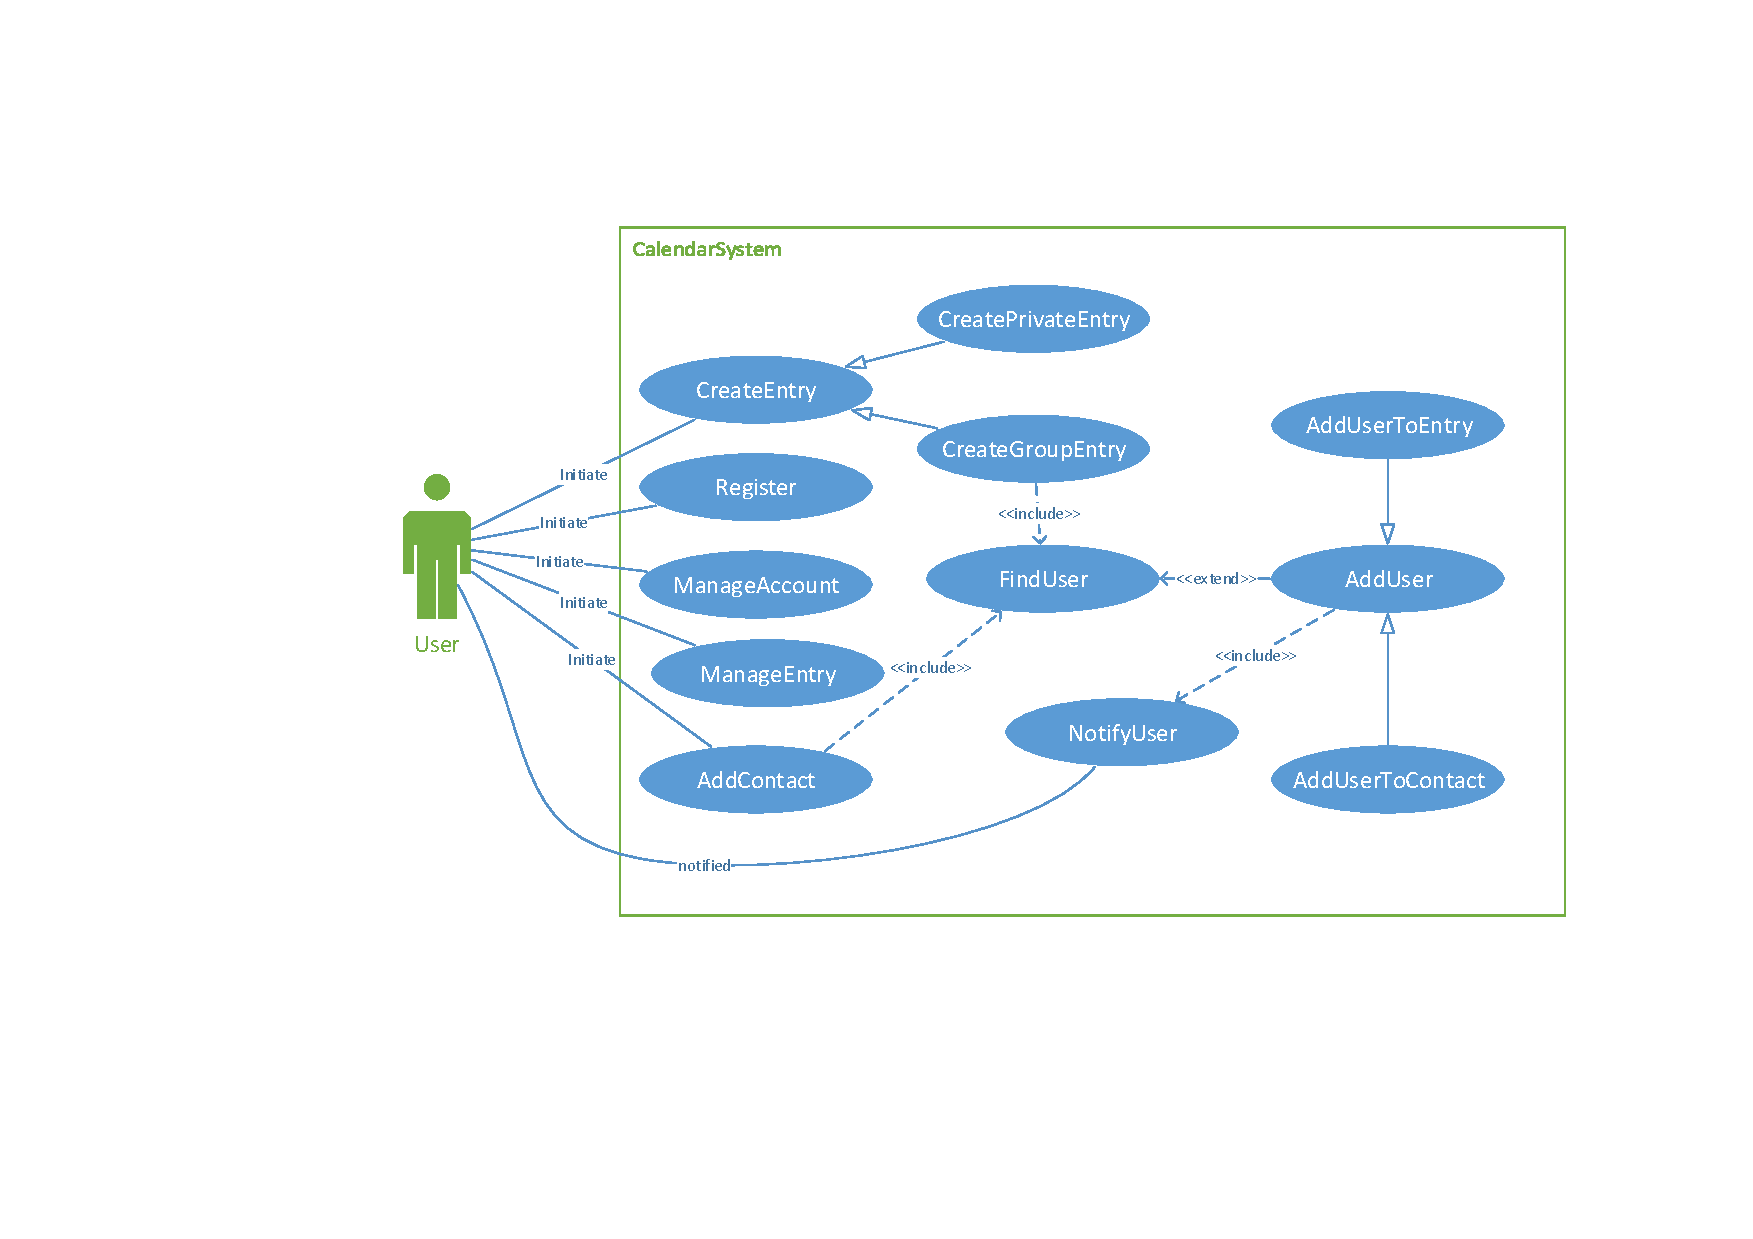
\includegraphics[scale = 0.8]{usecase}
\caption{Use case model}
\end{figure}
\pagebreak
\subsubsection{Use cases}

\begin{center}
    \begin{tabular}{ | l | p{10cm} |}
    \hline
    Use case name & CreateAccount \\ \hline
    Participating actors & User, Administrator \\ \hline
    Flow of events & \tabitem The Administrator activates the CreateNewAccount function from a computer. \\
    \mbox{} & \tabitem The calendar system presents a form to the Admin \\
    \mbox{} & \tabitem The Administrator fills out the form by filling out the different kinds of information about the User such as name, phone number, email and adds the user to one or more workgroups. \\
    \mbox{} & \tabitem The calendar system receives the form and notifies the Administrator that the form has been received and the account created. \\ \hline
    Entry condition & A request for a new calendar account has been made. Someone in the workplace contacts an Administrator and supplies the Administrator with the required information about the User. \\ \hline
    Exit condition & The account has been created for the User, and the User has been notified. \\ \hline
    \end{tabular}
\end{center}

\begin{center}
    \begin{tabular}{ | l | p{10cm} |}
    \hline
    Use case name & CreateEntry \\ \hline
    Participating actors & Initiated by User - communicates with User \\ \hline
    Flow of events & \tabitem The User activates the CreateNewEntry function from a computer. \\
    \mbox{} & \tabitem The calendar system presents a form to the User. \\
    \mbox{} & \tabitem The User fills out the form by filling out the different kinds of information about the new Entry such as name of entry, time, expected duration and optionally location. The User can then choose to add one or more participants (users) or workgroups (groups of users) to the Entry. \\
    \mbox{} & \tabitem The calendar system notifies all the users that the User has added them to an Entry. \\ \hline
    \mbox{} & \tabitem The calendar system further notifies the User that the form has been received that all Users have been notifed and the Entry created. \\ \hline
    Entry condition & A user chooses to create a new Entry, opens the program from a computer and logs into the calendar system. \\ \hline
    Exit condition & The Entry has been created and the User has been notified of this. Furthermore all invited users have been notified and their respective calendars have been updated. \\ \hline
    \end{tabular}
\end{center}

\begin{center}
    \begin{tabular}{ | l | p{10cm} |}
    \hline
    Use case name & SetUpSync \\ \hline
    Participating actors & User \\ \hline
    Flow of events & \tabitem The User activates the SetUpSync function from a computer. \\
    \mbox{} & \tabitem The calendar system presents a form to the User. \\
    \mbox{} & \tabitem The User fills out the form by choosing one of the supported external calendars (such as google calendar, iCal) to synchronize with. The User then provides the calendar system with the username and password for the external calendar system. \\ 
    \mbox{} & \tabitem The calendar system receives the form and notifies the User that the form has been received and the Calendars are in the process of being synchronized. \\
    \mbox{} & \tabitem Finally the calendar system notifies the user that the synchronization is finished. \\
    \hline
    Entry conditions & A user who already has an existing external calendar chooses to set up a synchronization with it, opens the program from a computer and logs into the calendar system. \\ \hline
    Exit condition & The calendar system has imported all entries from the external calendar and has set up the chosen synchronization time interval with the external calendar. \\
    \hline
    \end{tabular}
\end{center}
\pagebreak
\subsection{Object model}
The models below shows a static view of the proposed calendar system with its classes shown as blue squares.
\begin{figure}[h]
\centering
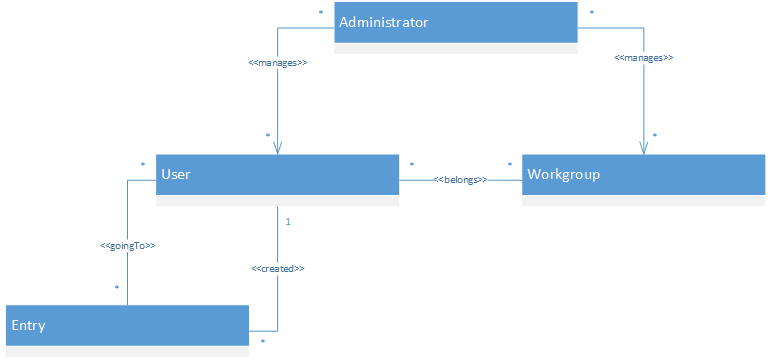
\includegraphics[scale = 0.6]{class21}
\caption{Class diagram, showing entity relations}
\end{figure}
\begin{figure}[h]
\centering
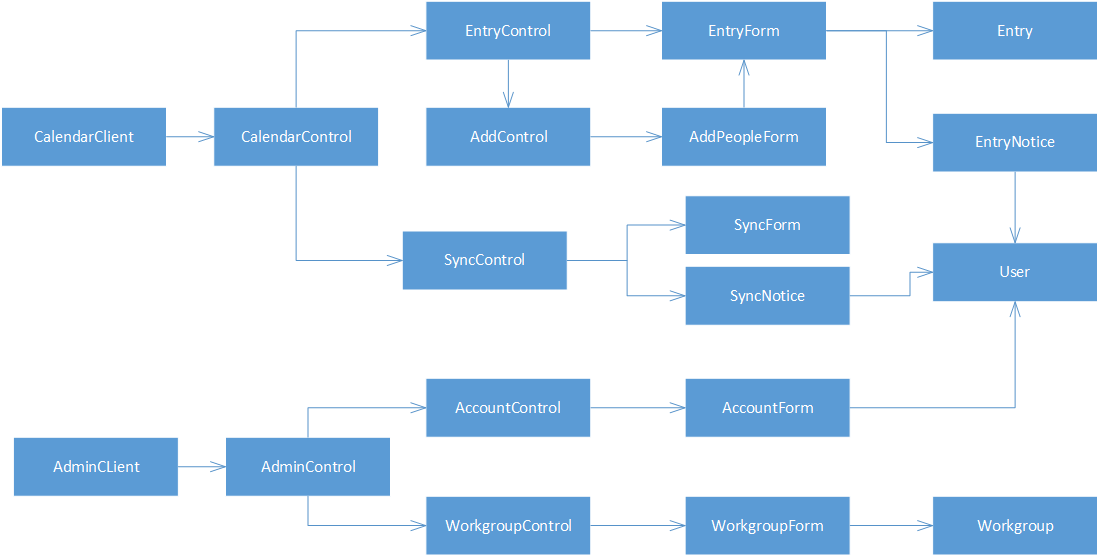
\includegraphics[scale = 0.5]{class22}
\pagebreak
\caption{Class diagram, showing relations between control, boundary and entity objects}
\end{figure}
\pagebreak
\subsection{Dynamic models}
Below is a statemachine diagram for an entry, showing which states it goes through.
\begin{figure}[h]
\centering
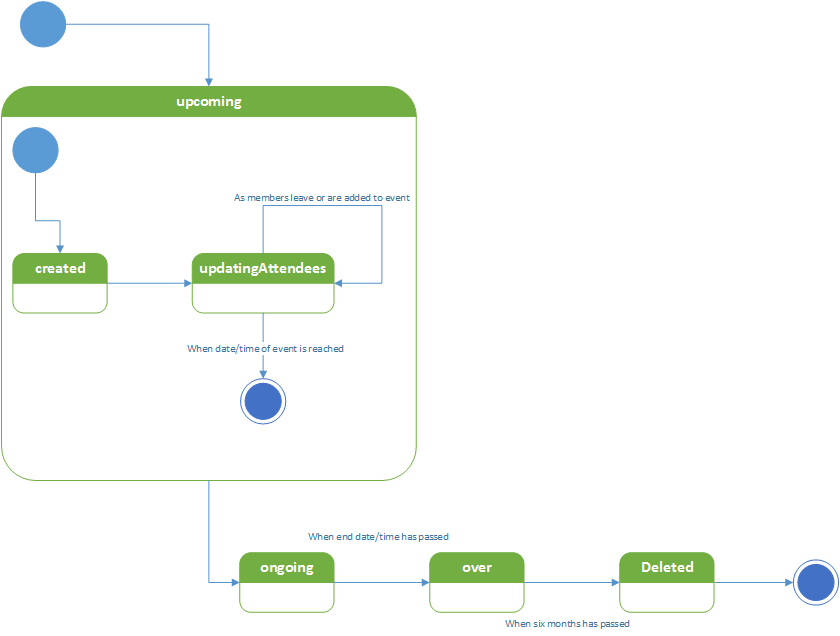
\includegraphics[scale = 0.5]{statemachine}
\caption{State machine diagram - entry}
\end{figure}
\pagebreak
\linebreak
The models below show two squence diagram of the use cases CreateEntry and CreateAccount. They show how the proposed calendar system will behave on runtime when creating an entry and creating an account.
\begin{figure}[ht]
\centering
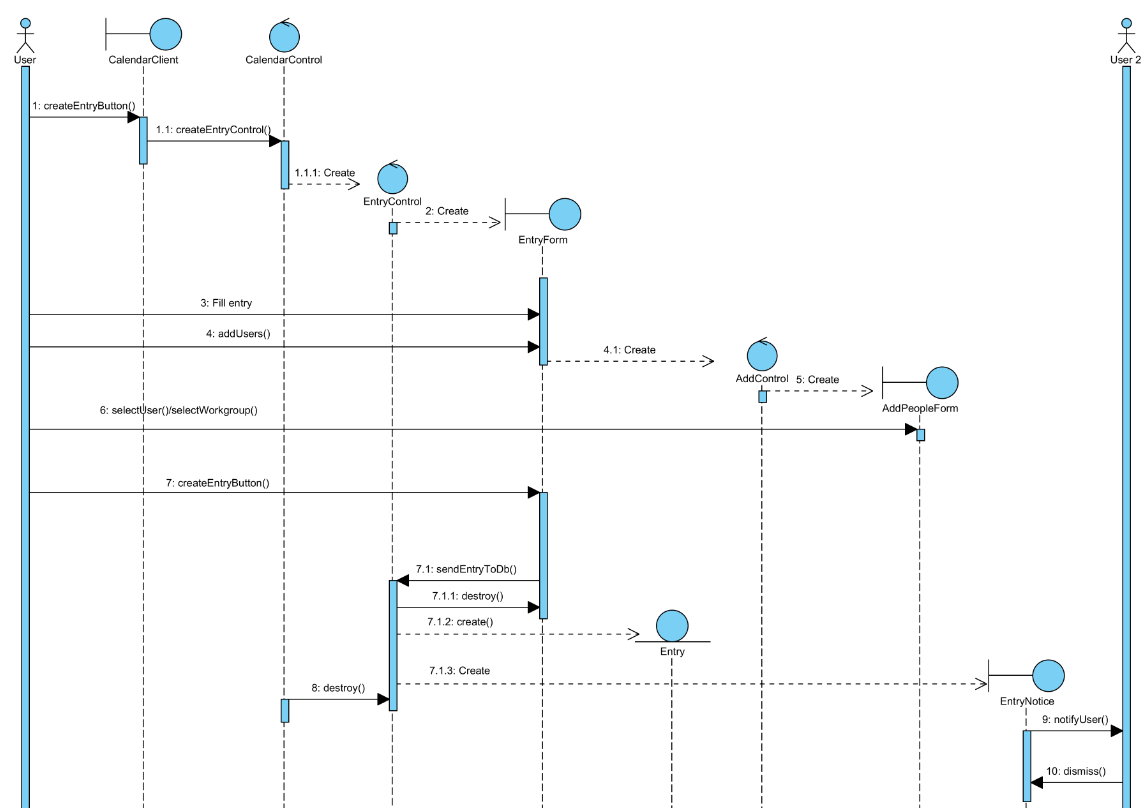
\includegraphics[scale = 0.6]{sequenceDiagram2}
\caption{Sequence diagram - CreateEntry}
\end{figure}
\pagebreak
\begin{figure}[h]
\centering
\includegraphics[scale = 0.6]{sequenceDiagram1}
\caption{Sequence diagram - CreateAccount}
\end{figure}